\documentclass[11pt, a4paper]{article}
\usepackage{pdfpages}
\usepackage{parallel}
\usepackage[T2A]{fontenc}
\usepackage{ucs}
\usepackage[utf8x]{inputenc}
\usepackage[polish,english,russian]{babel}
\usepackage{hyperref}
\usepackage{rotating}
\usepackage[inner=2cm,top=1.8cm,outer=2cm,bottom=2.3cm,nohead]{geometry}
\usepackage{listings}
\usepackage{graphicx}
\usepackage{wrapfig}
\usepackage{longtable}
\usepackage{indentfirst}
\usepackage{array}
\usepackage{tikzsymbols}
\usepackage{soul}
\usepackage[ruled,vlined]{algorithm2e}
%\counterwithout{figure}{section} 

\usepackage{url}
\makeatletter
\g@addto@macro{\UrlBreaks}{\UrlOrds}
\makeatother

\newcolumntype{P}[1]{>{\raggedright\arraybackslash}p{#1}}
\frenchspacing
\usepackage{fixltx2e} %text sub- and superscripts
\usepackage{icomma} % коскі ў матэматычным рэжыме
\PreloadUnicodePage{4}

\newcommand{\longpage}{\enlargethispage{\baselineskip}}
\newcommand{\shortpage}{\enlargethispage{-\baselineskip}}

\def\switchlang#1{\expandafter\csname switchlang#1\endcsname}
\def\switchlangbe{
\let\saverefname=\refname%
\def\refname{Літаратура}%
\def\figurename{Іл.}%
}
\def\switchlangen{
\let\saverefname=\refname%
\def\refname{References}%
\def\figurename{Fig.}%
}
\def\switchlangru{
\let\saverefname=\refname%
\let\savefigurename=\figurename%
\def\refname{Литература}%
\def\figurename{Рис.}%
}

\hyphenation{admi-ni-stra-tive}
\hyphenation{ex-pe-ri-ence}
\hyphenation{fle-xi-bi-li-ty}
\hyphenation{Py-thon}
\hyphenation{ma-the-ma-ti-cal}
\hyphenation{re-ported}
\hyphenation{imp-le-menta-tions}
\hyphenation{pro-vides}
\hyphenation{en-gi-neering}
\hyphenation{com-pa-ti-bi-li-ty}
\hyphenation{im-pos-sible}
\hyphenation{desk-top}
\hyphenation{elec-tro-nic}
\hyphenation{com-pa-ny}
\hyphenation{de-ve-lop-ment}
\hyphenation{de-ve-loping}
\hyphenation{de-ve-lop}
\hyphenation{da-ta-ba-se}
\hyphenation{plat-forms}
\hyphenation{or-ga-ni-za-tion}
\hyphenation{pro-gramming}
\hyphenation{in-stru-ments}
\hyphenation{Li-nux}
\hyphenation{sour-ce}
\hyphenation{en-vi-ron-ment}
\hyphenation{Te-le-pathy}
\hyphenation{Li-nux-ov-ka}
\hyphenation{Open-BSD}
\hyphenation{Free-BSD}
\hyphenation{men-ti-on-ed}
\hyphenation{app-li-ca-tion}

\def\progref!#1!{\texttt{#1}}
\renewcommand{\arraystretch}{2} %Іначай формулы ў матрыцы зліпаюцца з лініямі
\usepackage{array}

\def\interview #1 (#2), #3, #4, #5\par{

\section[#1, #3, #4]{#1 -- #3, #4}
\def\qname{LVEE}
\def\aname{#1}
\def\q ##1\par{{\noindent \bf \qname: ##1 }\par}
\def\a{{\noindent \bf \aname: } \def\qname{L}\def\aname{#2}}
}

\def\interview* #1 (#2), #3, #4, #5\par{

\section*{#1\\{\small\rm #3, #4. #5}}
\ifx\ParallelWhichBox\undefined%
    \addcontentsline{toc}{section}{#1, #3, #4}%
\else%
\ifnum\ParallelWhichBox=0%
    \addcontentsline{toc}{section}{#1, #3, #4}%
\fi\fi%

\def\qname{LVEE}
\def\aname{#1}
\def\q ##1\par{{\noindent \bf \qname: ##1 }\par}
\def\a{{\noindent \bf \aname: } \def\qname{L}\def\aname{#2}}
}

\newcommand{\interviewfooter}[1]{
\vskip 1em
\noindent \textit{#1}
}


\begin{document}

\title{1983 "--- Logitech LOGIMOUSE P5}
\date{}
\maketitle

Мышь LOGIMOUSE P5 была выпущена в 1983 году. Это второй по счету манипулятор фирмы Logitech (после P4, выпуск которого продолжился одновременно с P5). P5 был удешевленной моделью (отпускная цена различалась на \$100) и предназначался в первую очередь для поставок ОЕМ.
Но главной особенностью P5 является кардинально отличающийся внешний вид (рис. \ref{fig:LogimouseP5Pic}). 

\begin{figure}[h]
   \centering
    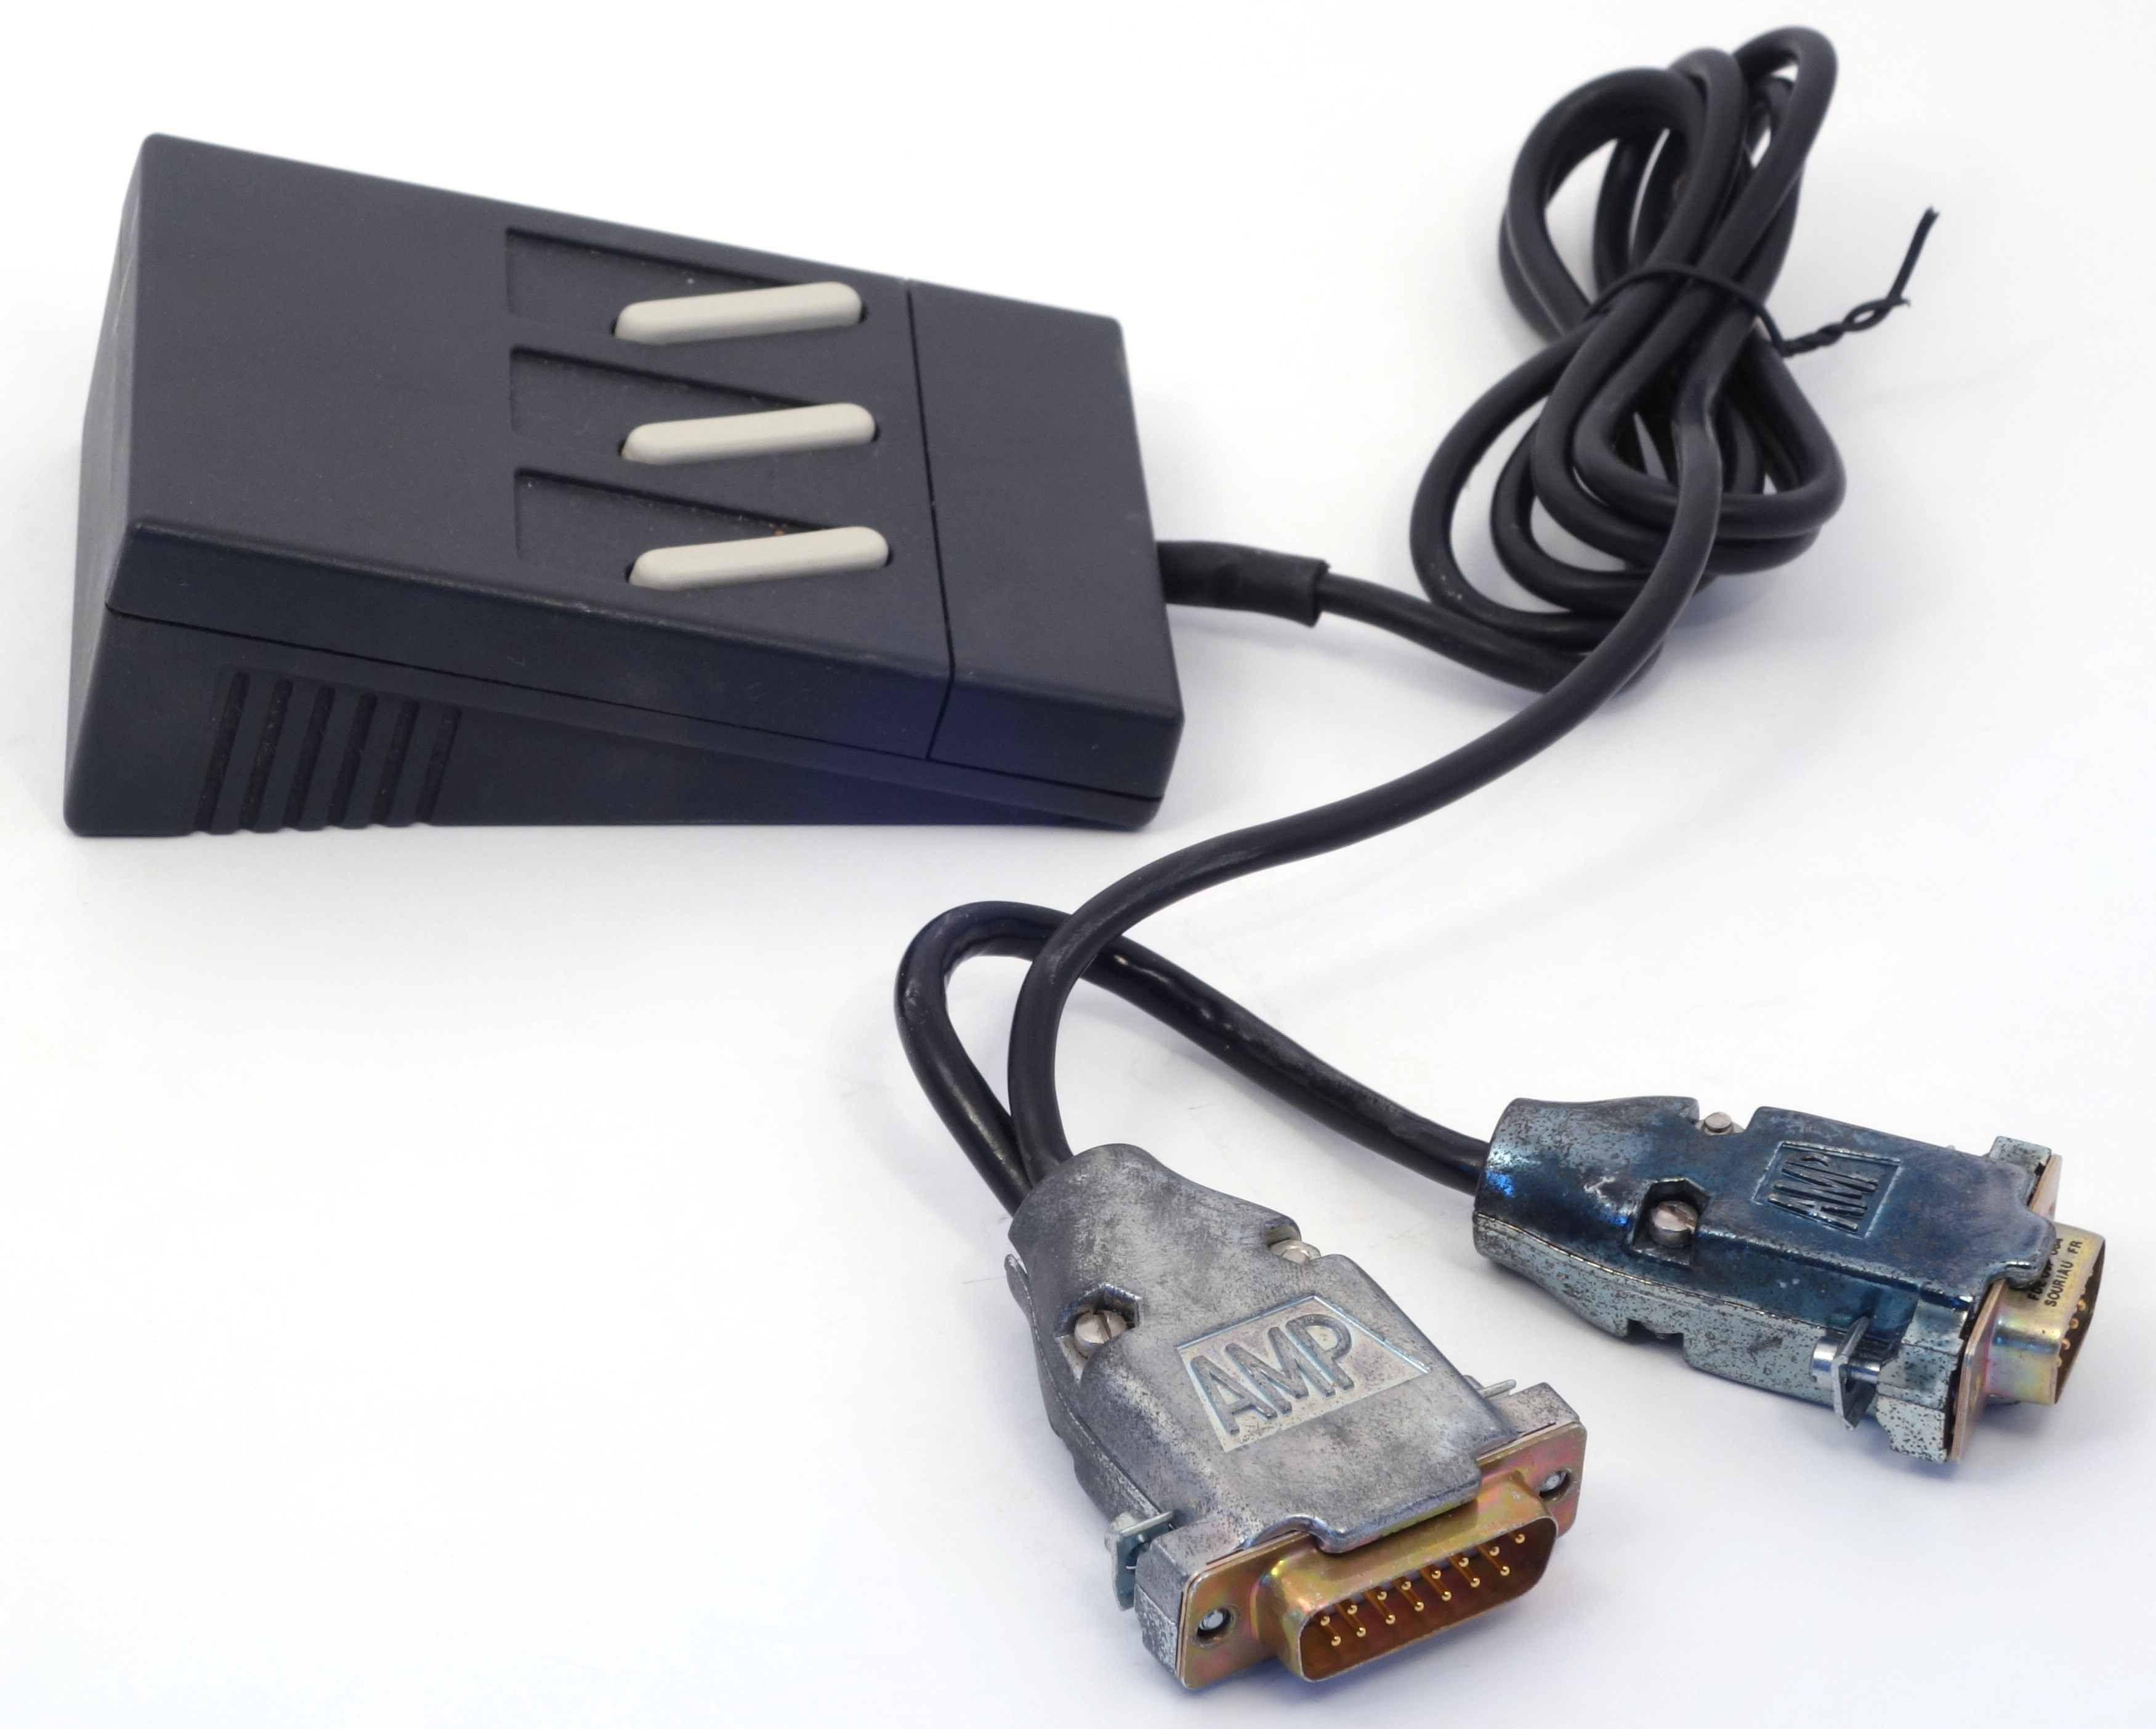
\includegraphics[scale=0.35]{1983_logitech_logimouse_p5/pic_30.jpg}
    \caption{LOGIMOUSE P5, вид спереди}
    \label{fig:LogimouseP5Pic}
\end{figure}

Мышь имеет вызывающе дизайнерскую наружность, хотя в 1983 году этого понятия еще не существовало: на черном призматическом корпусе с обратным наклоном диагонально располагаются три узкие белые кнопки. На нижней стороне присутствуют четыре белые опоры с низким коэффициентом трения (одновременно это крепления печатной платы), и шар, выполненный из матового металла (рис. \ref{fig:LogimouseP5TopAndBottom}). Можно отметить съемное поворотное кольцо на защелках, позволяющее извлечь шар для удаления собравшегося мусора и чистки роликов. В LOGIMOUSE P4 и других мышах первой половины 80-х годов кольцо требовалось отвинтчивать с помощью отвертки; таким образом, это один из первых случаев (наряду с мышью Apple Lisa того же года выпуска) применения поворотного кольца, ставшего впоследствии стандартом.

\begin{figure}[h]
    \centering
    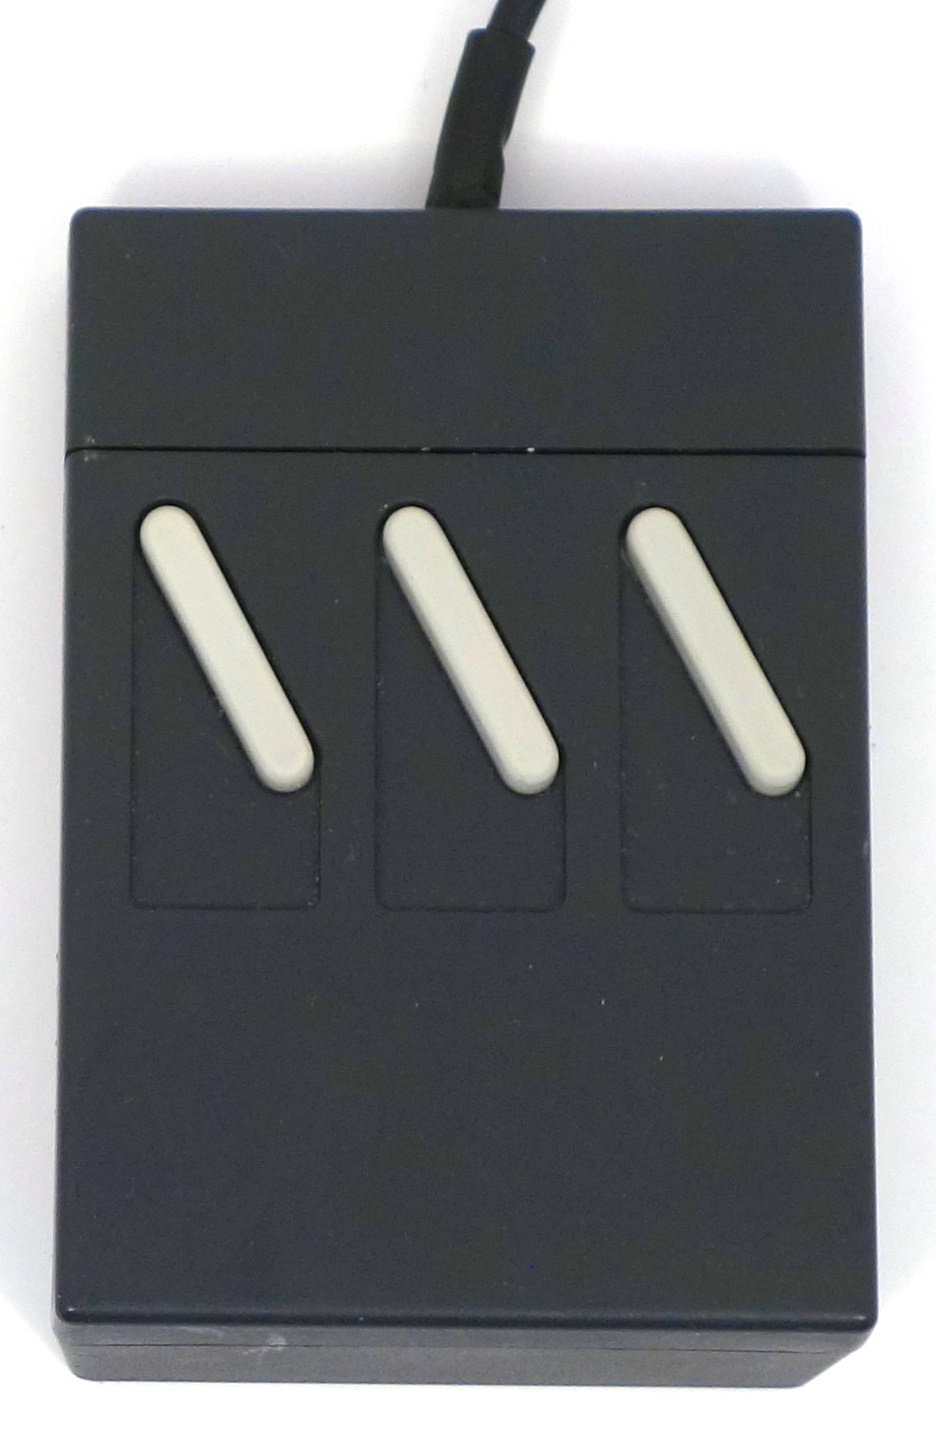
\includegraphics[scale=0.4]{1983_logitech_logimouse_p5/top_30.jpg}
    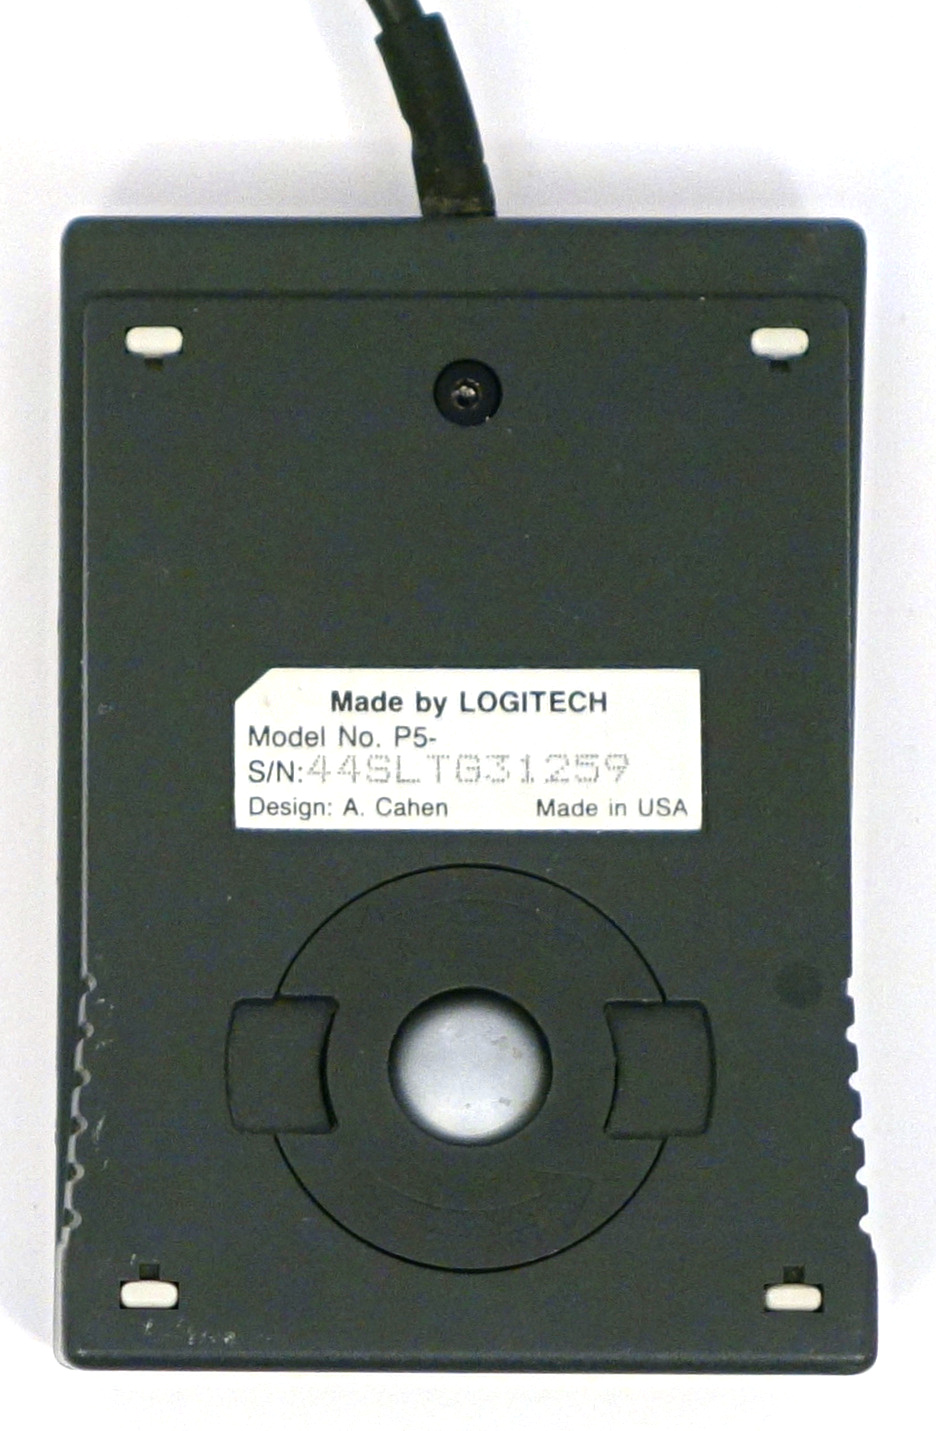
\includegraphics[scale=0.4]{1983_logitech_logimouse_p5/bottom_30.jpg}
    \caption{LOGIMOUSE P5, вид сверху и снизу}
    \label{fig:LogimouseP5TopAndBottom}
\end{figure}

Судя по кабелю с двумя разъемами, это мышь от FutureNet "--- рабочей станции для САПР микроэлектроники. Компьютер представлял собой классическую IBM PC с монохромным текстовым видеоадаптером и дополнительной графической платой разрешением 640x360 пикселей, и пятнадцатиконтактный разъем на кабеле мыши использовался, чтобы соединить выход монохромного видеоадаптера IBM и графическую плату. Такое решение позволяло попеременно использовать дисплей для текстового вывода и для вывода графики редактором схем \cite{futurenet}.

\begin{figure}[h]
    \centering
    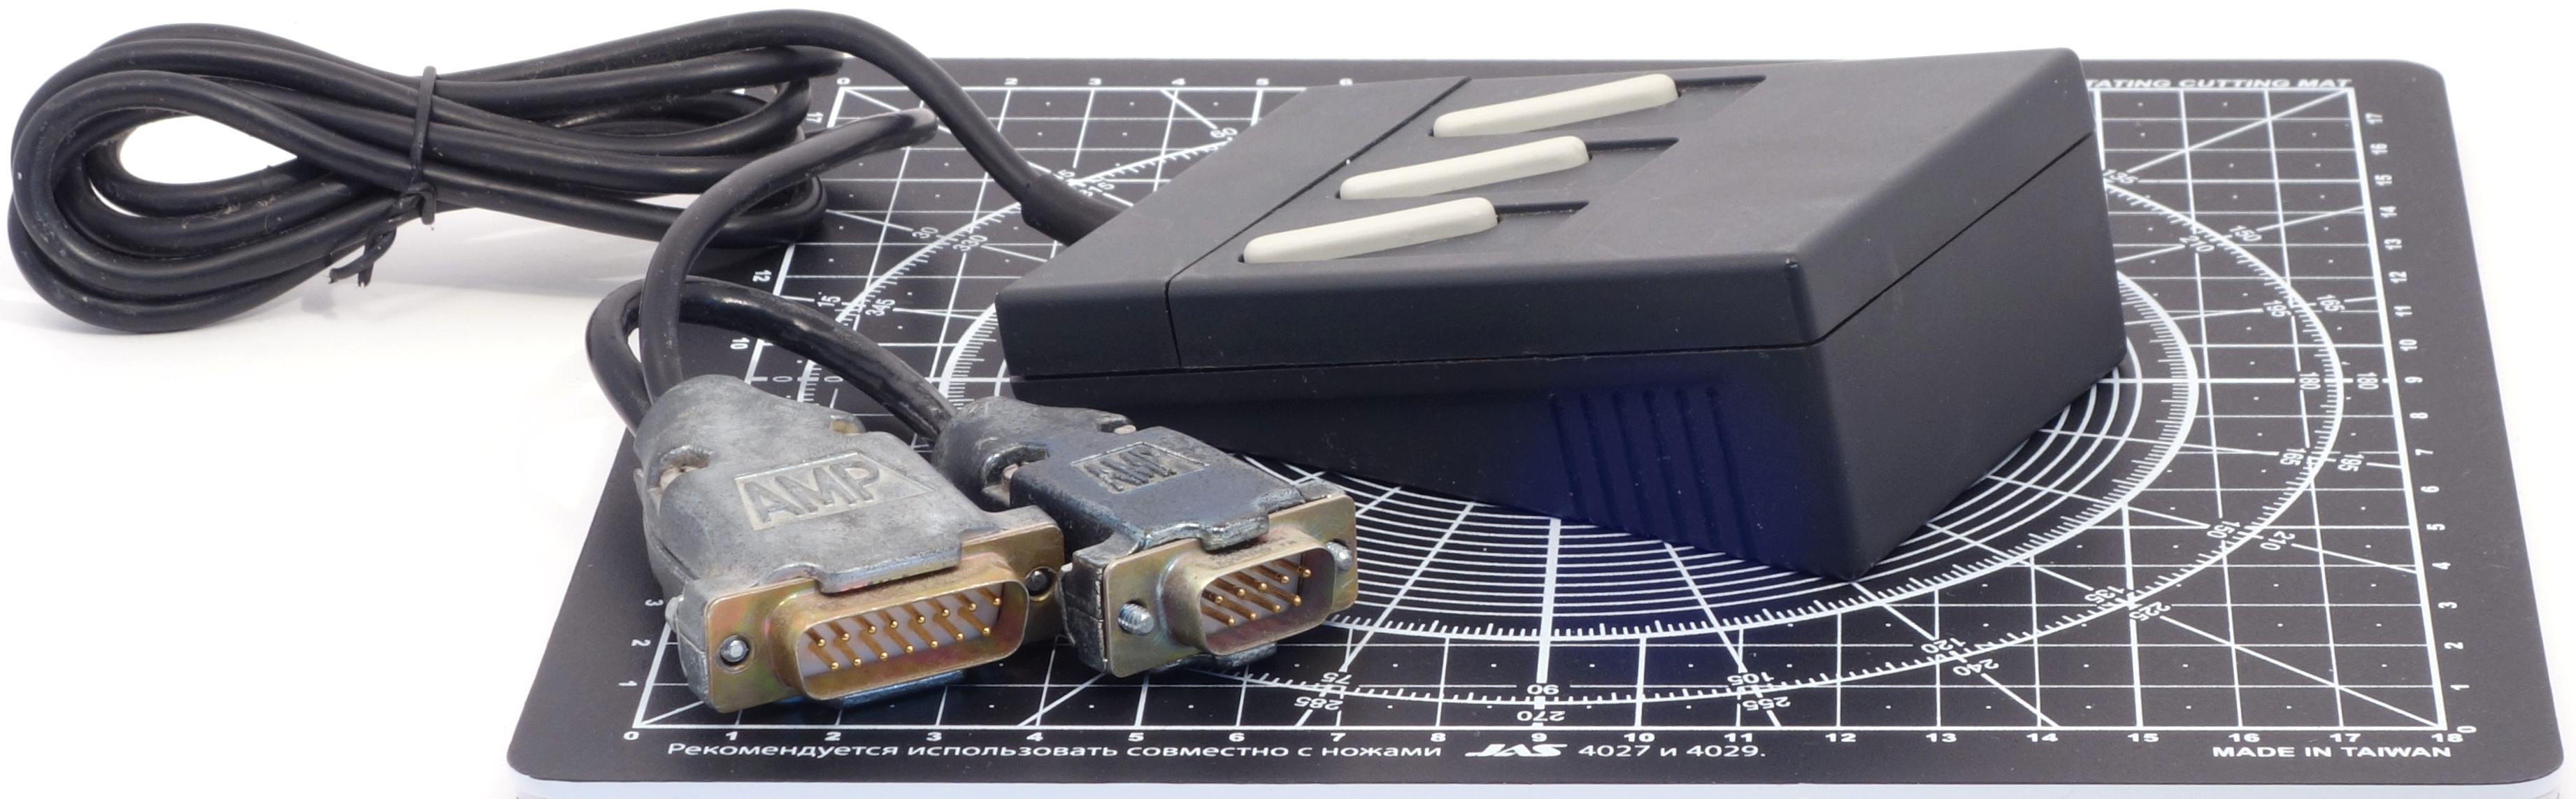
\includegraphics[scale=0.5]{1983_logitech_logimouse_p5/size_30.jpg}
    \caption{LOGIMOUSE P5 на размерном коврике с шагом сетки 1~см}
    \label{fig:LogimouseP5Size}
\end{figure}

Мышь имеет размеры, типичные для мышей 1980-х годов (рис. \ref{fig:LogimouseP5Size}). Фактически, ее габариты близки к более поздней модели Logitech P7 и ее наиболее массовой разновидности, C7. Что касается эргономики, то очевидно, что призматический корпус и диагональные узкие кнопки сказались на ней весьма негативно: при расположении пальцев вдоль кнопок ладонь рискует опереться на торчащий на угол корпуса, а расположении ладони вдоль линий корпуса улучшает ситуацию лишь незначительно, взамен осложняя нажатие на и без того неудобные кнопки (рис. \ref{fig:LogimouseP5Hand}).

\begin{figure}[h]
    \centering
    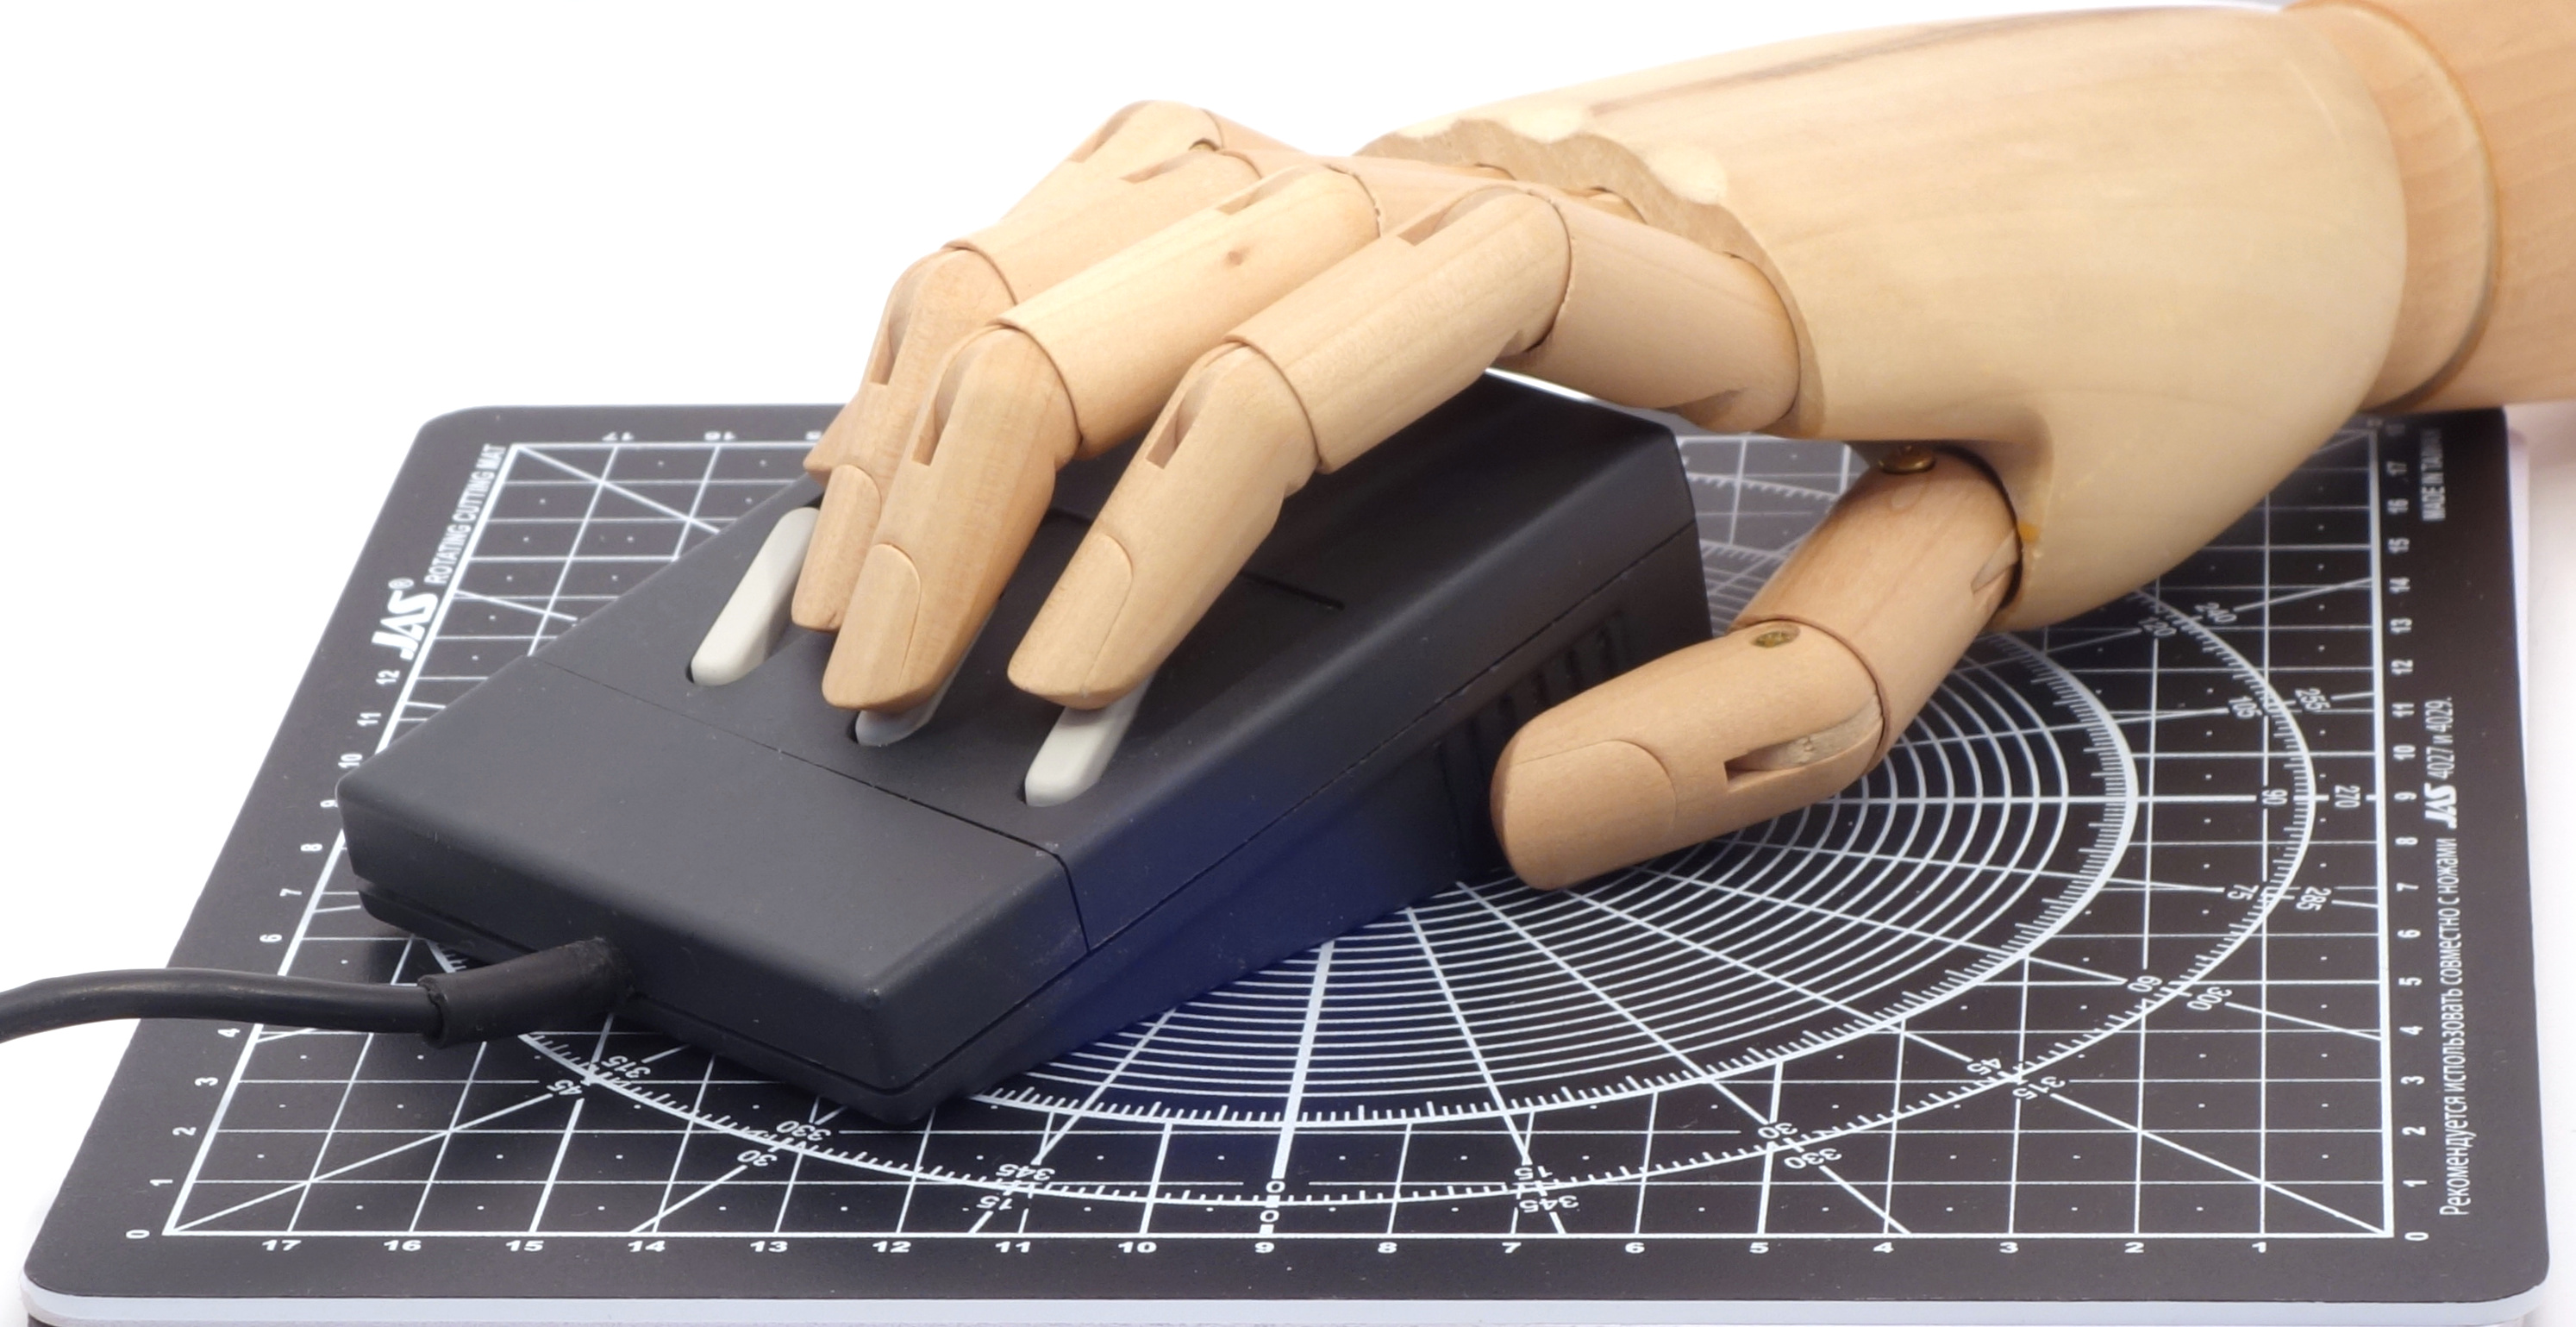
\includegraphics[scale=0.5]{1983_logitech_logimouse_p5/hand_30.jpg}
    \caption{LOGIMOUSE P5 с моделью руки человека}
    \label{fig:LogimouseP5Hand}
\end{figure}

В электрическом плане P5 аналогична мыши Logitech P4, но имеет меньшее разрешение (200 DPI против 381 DPI). В качестве дополнительного аксессуара обе мыши могли комплектоваться специальным адаптером-переходником LogiMate, который позволял подключить мышь не к отдельному адаптеру с шинным интерфейсом, а в разрыв кабеля клавиатуры. При таком подключении перемещение мыши приводило к генерации кодов нажатий клавиш управления курсором: в стандартном режиме разрешение составляло 12 нажатий клавиш на дюйм по горизонтали и 6 нажатий по вертикали, что было рассчитано на работу в текстовом режиме 80x25 символов. В \cite{logimouse} отмечается, что использование мыши в стандартном режиме позволяло перемещать курсор в текстовом редакторе в семь раз быстрее, чем соответствующие клавиши на клавиатуре (однако требовалось привыкнуть к тому, что в результате небольшого промаха пользователя за крайней правой позицией курсор текстового редактора неизменно перескакивал на левую позицию следующей строки). По очевидным причинам для использования мыши не требовался драйвер; однако его применение давало возможность дополнительных настроек "--- например, позволяло выставлять разрешение переходника LogiMate в диапазоне 1--100 нажатий на дюйм, а также переназначить действие клавиш мыши (по-умолчанию генерировались коды клавиш F8, F9 и F10).

 \begin{figure}[h]
    \centering
    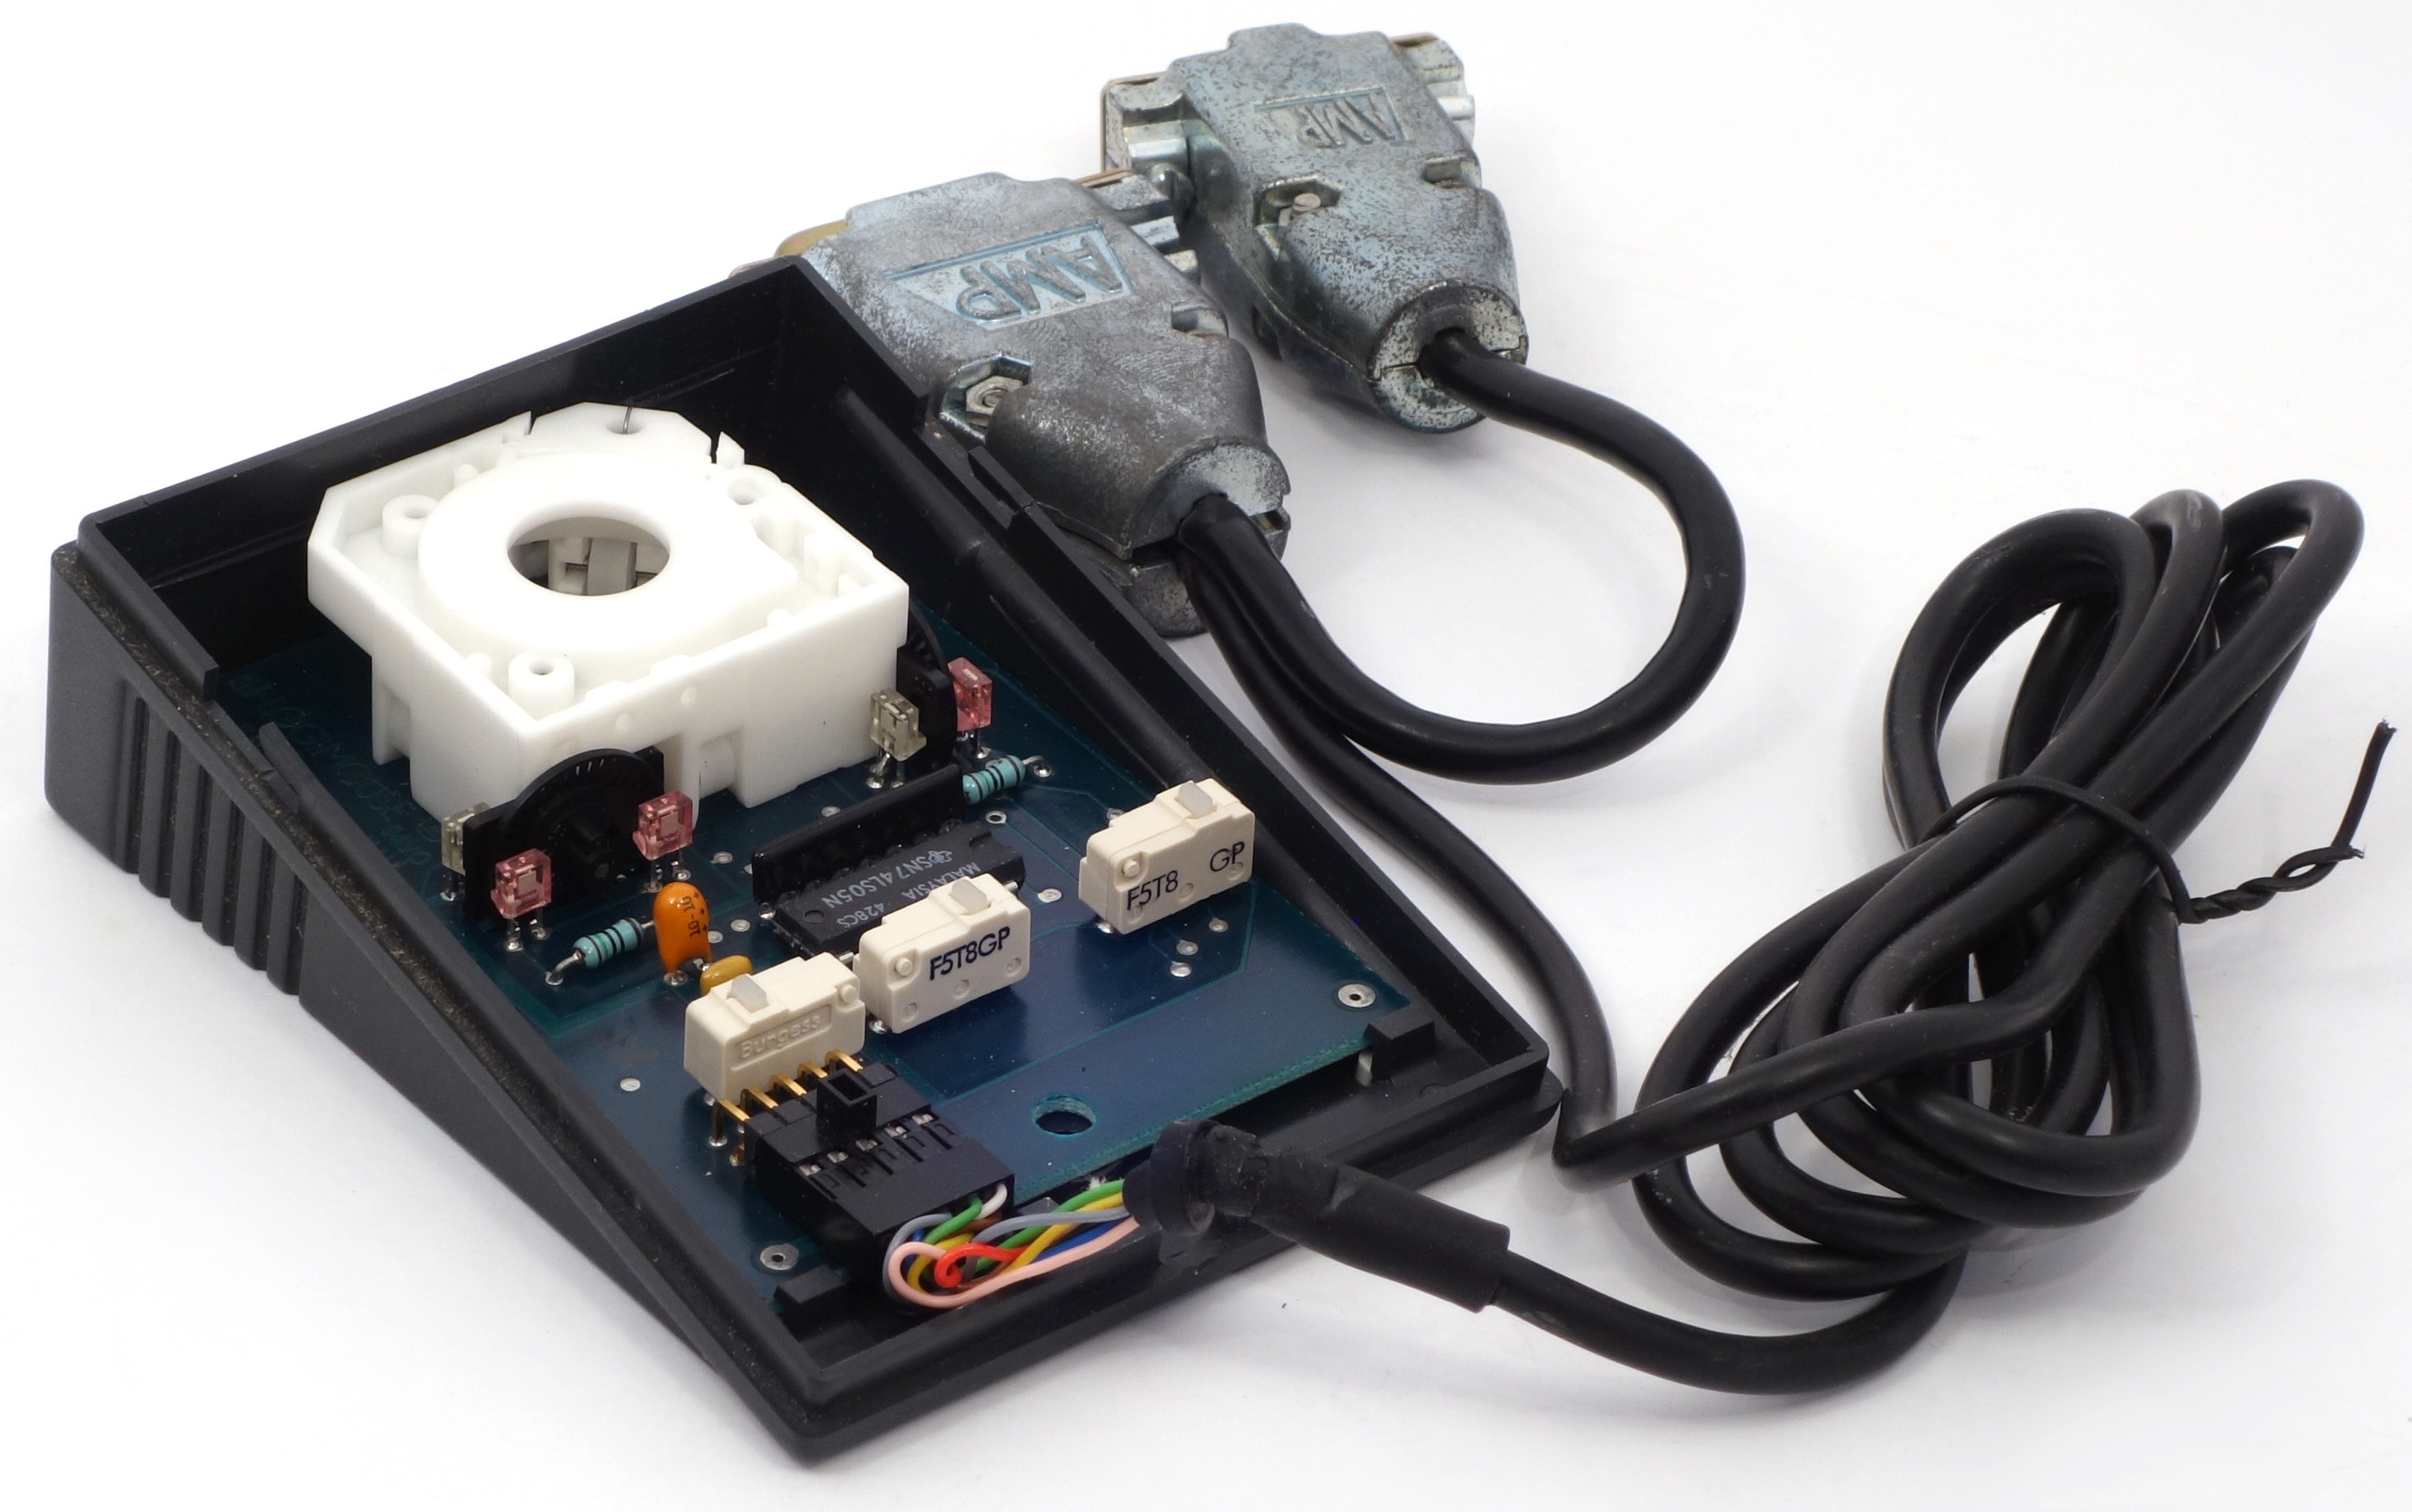
\includegraphics[scale=0.7]{1983_logitech_logimouse_p5/inside_30.jpg}
    \caption{LOGIMOUSE P5 в разобранном виде}
    \label{fig:LogimouseP5Inside}
\end{figure}

Внутреннее устройство мыши показано на рис. \ref{fig:LogimouseP5Inside}. В мыши использованы оптомеханические энкодеры. Оптопары и диск оптического прерывателя очень похожи на соответствующие детали в мышах 90-х годов (можно считать это первой их подобной реализацией). Отличительной особенностью энкодера (как и в модели P4) является дополнительная неподвижная маска, уменьшавшая площадь засветки.

\begin{thebibliography}{9}
\bibitem {logimouse} J. Taylor. Faster then a speeding cursor key. // PC Magazine, V. 3, No. 2, February 7, 1984. - p. 243-245 \url{https://archive.org/details/PC-Mag-1984-02-07/page/n243/mode/2up}
\bibitem {futurenet} M. Holley. Logitech Logimouse Cable 1983 \url{https://commons.wikimedia.org/wiki/File:Logitech_Logimouse_Cable_1983.jpg}
\end{thebibliography}
\end{document}
